\documentclass[12pt,a4paper]{article}

\usepackage[utf8]{inputenc}
\usepackage[T1]{fontenc}
\usepackage{lmodern}
\usepackage[margin=1in]{geometry}
\usepackage{array}
\usepackage{booktabs}
\usepackage{enumitem}
\usepackage{graphicx}
\usepackage{hyperref}
\usepackage{xcolor}

\hypersetup{
  colorlinks=true,
  linkcolor=blue,
  urlcolor=blue
}

\setlist[itemize]{itemsep=3pt, topsep=4pt}
\setlist[enumerate]{itemsep=3pt, topsep=4pt}

\title{\textbf{Geometry Studio}\\Computer Graphics 3D Project Report}
\author{Student ID: \textit{replace with your student ID}}
\date{May 29, 2026}

\begin{document}

\maketitle

\begin{abstract}
Geometry Studio is an interactive WebGL2 application for demonstrating core
computer graphics concepts in three-dimensional space. The project implements
primitive geometry generation, model loading, solid/point/line rendering modes,
perspective projection controls, affine transformations, lighting, shadows,
texture mapping, animation, scene persistence, post-processing, and an
evaluator-focused tour. The application is built with Three.js, TypeScript,
Vite, and a keyframe timeline editor, and is packaged as a static release that
can be served locally for grading.
\end{abstract}

\tableofcontents
\newpage

\section{Project Overview}

The goal of this project is to build a practical 3D graphics studio rather than
a collection of isolated demonstrations. The application allows users to create
objects, inspect their rendering modes, transform them interactively, adjust the
camera projection, configure lights and shadows, apply textures, import external
models, and run animations.

The project is designed for two audiences:
\begin{itemize}
  \item \textbf{Course evaluators}, who need to verify that every assignment
  requirement is implemented clearly.
  \item \textbf{Students and developers}, who need a maintainable source
  structure that demonstrates how a real-time graphics application is organized.
\end{itemize}

\section{Technology Stack}

\begin{table}[h]
\centering
\begin{tabular}{>{\bfseries}p{0.28\linewidth}p{0.62\linewidth}}
\toprule
Technology & Purpose \\
\midrule
Three.js 0.184.0 & WebGL2 rendering, geometry, materials, lighting, shadows, controls, loaders, and post-processing. \\
TypeScript 6.0.3 & Static typing and safer long-term source maintenance. \\
Vite 8.0.14 & Development server and static production build. \\
Lucide & UI icon system. \\
Playwright & Browser smoke tests for release validation. \\
animation-timeline-js 2.3.5 & Canvas-based visual timeline control for transform keyframes. \\
pdflatex & English report generation from LaTeX source. \\
\bottomrule
\end{tabular}
\caption{Main technologies used in the project.}
\end{table}

\section{Implemented Requirements}

\subsection{3D Geometry}

The application supports the required primitive shapes:
\begin{itemize}
  \item Box / Cube
  \item Sphere
  \item Cone
  \item Cylinder
  \item Wheel / Torus
  \item Teapot
\end{itemize}

Additional self-researched shapes are also included:
\begin{itemize}
  \item Torus Knot
  \item Tube Curve
  \item Tetrahedron, Octahedron, Dodecahedron, and Icosahedron
  \item Parametric Surface
  \item Extruded Star
  \item Built-in sample drone model for model-loading demonstrations
\end{itemize}

Primitive geometry is generated using Three.js buffer geometries and normalized
so that objects are centered in the scene and placed naturally on the ground
plane. This makes the scene easier to inspect and makes object transformations
more predictable.

\subsection{Rendering Modes}

Each object can be displayed in three required modes:
\begin{itemize}
  \item \textbf{Solid}: rendered as a mesh with material and lighting.
  \item \textbf{Points}: rendered as vertices using \texttt{THREE.Points}.
  \item \textbf{Lines}: rendered using \texttt{WireframeGeometry} and
  \texttt{LineSegments}.
\end{itemize}

The line mode deliberately uses a real wireframe geometry instead of a single
\texttt{Line} object. This avoids incomplete edge rendering on complex geometry
and imported models.

\subsection{Perspective Projection}

The project uses \texttt{THREE.PerspectiveCamera}. The user can adjust:
\begin{itemize}
  \item Camera position on the X, Y, and Z axes
  \item Field of view
  \item Near clipping plane
  \item Far clipping plane
\end{itemize}

Camera presets are provided for front, top, isometric, and reset views. A camera
frustum helper can be enabled to make the projection volume visible during
evaluation.

\subsection{Affine Transformations}

Affine transformations are implemented with \texttt{TransformControls}. The
selected object can be translated, rotated, or scaled using:
\begin{itemize}
  \item On-screen transform gizmos
  \item Keyboard shortcuts: T, R, and S
  \item Numeric inspector fields for X, Y, and Z values
  \item World-space and local-space transform modes
\end{itemize}

Each scene object is wrapped in a \texttt{THREE.Group}, which provides a stable
transform root even when the object's internal visual representation changes
between solid, point, and line modes.

\subsection{Lighting and Shadows}

The lighting system includes:
\begin{itemize}
  \item Ambient light for global illumination
  \item Directional light to simulate sunlight
  \item Point light
  \item Spot light
\end{itemize}

The user can control light color, intensity, position, helpers, shadow state,
and a light sweep animation. Five direct-lighting presets are provided:
Studio, Product, Dramatic, Soft, and Night. These presets combine ambient,
directional, point, and spot lights into complete rigs so the evaluator can
compare neutral, product, dramatic, soft-fill, and low-key lighting without
manually editing every light.

The renderer uses configurable shadow-map quality, \texttt{PCFSoftShadowMap},
and a shadow-receiving ground plane to make shadows visible during grading.

\subsection{Texture Mapping}

The project includes built-in procedural texture presets:
\begin{itemize}
  \item Checker
  \item UV grid
  \item Grid
\end{itemize}

Users can also upload bitmap images from their computer. Uploaded textures are
loaded through \texttt{TextureLoader}, assigned to the selected material, and
configured with sRGB color space. Repeat, offset, and rotation controls can be
adjusted from the inspector and can also be keyed in the timeline.

\subsection{Model Loading}

The application supports external model import in the following formats:
\begin{itemize}
  \item GLB / GLTF
  \item OBJ
  \item STL
\end{itemize}

The import pipeline uses \texttt{LoadingManager} for progress reporting and
clear error messages. Imported objects are normalized, centered, scaled to a
reasonable size, placed on the ground plane, and added to the same outliner and
transformation workflow as primitive objects. Drag-and-drop import is also
supported.

\subsection{Animation}

The application supports a keyframe-first animation workflow. Per-object preset
buttons generate editable timeline keyframes instead of hidden procedural
motion. The available presets are:
\begin{itemize}
  \item Spin
  \item Orbit
  \item Bounce
  \item Pulse
\end{itemize}

The project also includes a light sweep preset for demos; it is baked into light
position keyframes so the resulting motion is visible in the same timeline as
object motion.

The keyframe timeline provides a resizable bottom editing dock with a playhead,
timecode, duration, FPS, Work In/Out range, snapping, loop control, and tracks
for object transforms, object appearance, camera properties, and lights. Users
can add, delete, duplicate, copy, paste, drag, scrub, save, and reload
keyframes.
The \texttt{Set TRS} timeline command records the selected object's Position,
Rotation, and Scale together at the playhead, so a complete pose can be keyed at
\(t_0\), changed, and keyed again at \(t_1\) for pose-to-pose interpolation.
When the selected object has two or more Position keyframes, the viewport draws
a motion path: a curve for the sampled trajectory and points for the authored
key positions. This makes the animation relationship from an initial position
at time \(t_0\) to a later position at time \(t_1\) visible directly in the
scene, instead of only in the timeline row.
The left row labels select object, camera, and light tracks directly, and active
tracks can be disabled non-destructively to test motion or appearance changes
without deleting keyframes. Focus, Keyed, and All row filters keep dense scenes
manageable while preserving access to the active track. Object Position,
Rotation, and Scale tracks are expanded into X/Y/Z timeline rows for clearer
motion inspection while remaining vector tracks in the saved JSON document.
Each timeline row also
has a diamond key button, allowing users to key a property directly from its row
in the style of motion-graphics editors. Named timeline markers add cue points
for animation beats, camera moves, and demo sections.
Frame-accurate navigation is available through previous/next frame buttons and
keyboard shortcuts, while selected keyframes can be nudged one frame left or
right for precise retiming. A compact keyframe editor allows precise numeric
edits to keyframe time and vector or scalar values. Linear, Easy Ease, and Hold
interpolation are available through direct timeline buttons, synchronized with a
compact curve preview and F9-style keyboard shortcuts. The timeline also
provides an active-track value graph that samples the same runtime interpolation
function used by playback, so Hold, Linear, and Easy Ease segments shown in the
graph match the object, camera, light, or material values seen while scrubbing.
The graph draws key points on top of the curves and supports horizontal and
vertical dragging to retime a keyframe and edit a keyed channel value; each
graph drag is recorded as one undoable edit. Graph retiming follows the
timeline Snap setting, and Shift-dragging constrains the edit to the dominant
drag direction for more precise graph adjustments.
The editor stores rotation keyframes in readable Euler degrees and evaluates
rotation playback per axis, preserving authored full turns such as \(0^\circ\)
to \(360^\circ\).

\section{Advanced Features}

\subsection{Scene Persistence}

The application can save and load a typed JSON scene document. The document
stores:
\begin{itemize}
  \item Scene version and save time
  \item Object names, types, render modes, materials, colors, textures, and
  transforms
  \item Object animation settings
  \item Keyframe timeline settings, object tracks, and keyframe values
  \item Camera position, target, field of view, near plane, and far plane
  \item Display settings such as UI density, grid, axes, stats, and frustum helper
  \item Lighting configuration
\end{itemize}

External model binary data is not embedded into the JSON document. If a saved
scene references an imported model, the loader restores a built-in sample
placeholder so the scene workflow remains usable.

\subsection{Undo and Redo}

Undo and redo are implemented through a command-history system that stores
snapshots of the scene document. This allows the project to restore prior states
after changes such as object creation, deletion, material changes, render mode
changes, camera changes, lighting changes, and timeline keyframe edits.

\subsection{Keyframe Timeline Runtime}

The keyframe timeline is implemented as a separate editor layer and runtime
layer. The UI layer uses \texttt{animation-timeline-js} for visual keyframe rows,
selection, dragging, snapping, and playhead interaction. Geometry Studio owns the
actual scene timeline schema so saved JSON files remain stable and independent
from the UI library.

At runtime, transform and property tracks are evaluated directly from the saved
timeline document:
\begin{itemize}
  \item Position and Scale write vector values to the selected object.
  \item Rotation stores readable Euler degrees and converts them to radians at
  playback time, preserving full-turn animations.
  \item Hold, Linear, and Easy Ease interpolation are evaluated per keyframe
  segment, so mixed timing within a single track is supported.
\end{itemize}

If an object has active transform timeline tracks, timeline playback overrides
the older preset transform animation for that same object. This avoids ambiguous
motion and makes the evaluator-visible behavior deterministic.

\subsection{Rendering Lab}

The Rendering Lab exposes renderer controls directly in the inspector. It makes
the project clearer during grading because the evaluator can see that the main
viewport is a real-time WebGL raster renderer, not an offline ray tracer.

Implemented rendering controls include:
\begin{itemize}
  \item Tone mapping: ACES, Linear, Reinhard, or none
  \item Exposure
  \item Shadow quality: Low, Medium, High, and Ultra
  \item Generated PMREM environment lighting presets
  \item PBR material presets for Ceramic, Metal, Plastic, Glass, Clay, and
  texture comparison
  \item Post-processing toggles for FXAA, SSAO, Bloom, and Vignette
\end{itemize}

FXAA is used as a lightweight screen-space anti-aliasing pass at the end of the
composer chain. SSAO adds contact shading for depth perception, Bloom provides
glow for cinematic demos, and Vignette gives an optional composition effect.
These effects are optional and disabled conservatively by default so the release
remains responsive on typical evaluator hardware.

\subsection{Evaluation Tour}

The Evaluation Tour is designed specifically for grading. It creates a scene
that demonstrates:
\begin{itemize}
  \item Required primitive geometry
  \item Solid, point, and line rendering
  \item Perspective camera and frustum helper
  \item Affine transform workflow
  \item Ambient, spot, and shadowed lighting
  \item Texture mapping
  \item Model-loading workflow through the built-in sample model
  \item Multiple animation types
\end{itemize}

Toast messages appear in sequence to explain which requirement is being shown.

\subsection{Cinematic Demo and Screenshot Export}

The Cinematic Demo creates a visually stronger scene with different geometry,
materials, render modes, textures, and animations. The screenshot button exports
the current WebGL canvas as a PNG image.

\subsection{Telemetry}

The telemetry panel displays FPS, draw calls, triangles, lines, points, geometry
count, texture count, and object count. These values are based on
\texttt{renderer.info} and help demonstrate rendering cost during manual
evaluation.

\section{Captured Screenshots}

The following screenshots were captured from the static \texttt{Release/} build
served locally through \texttt{python3 -m http.server 8080}. They demonstrate
the final evaluator-facing interface and the major graphics features.

\begin{figure}[htbp]
\centering
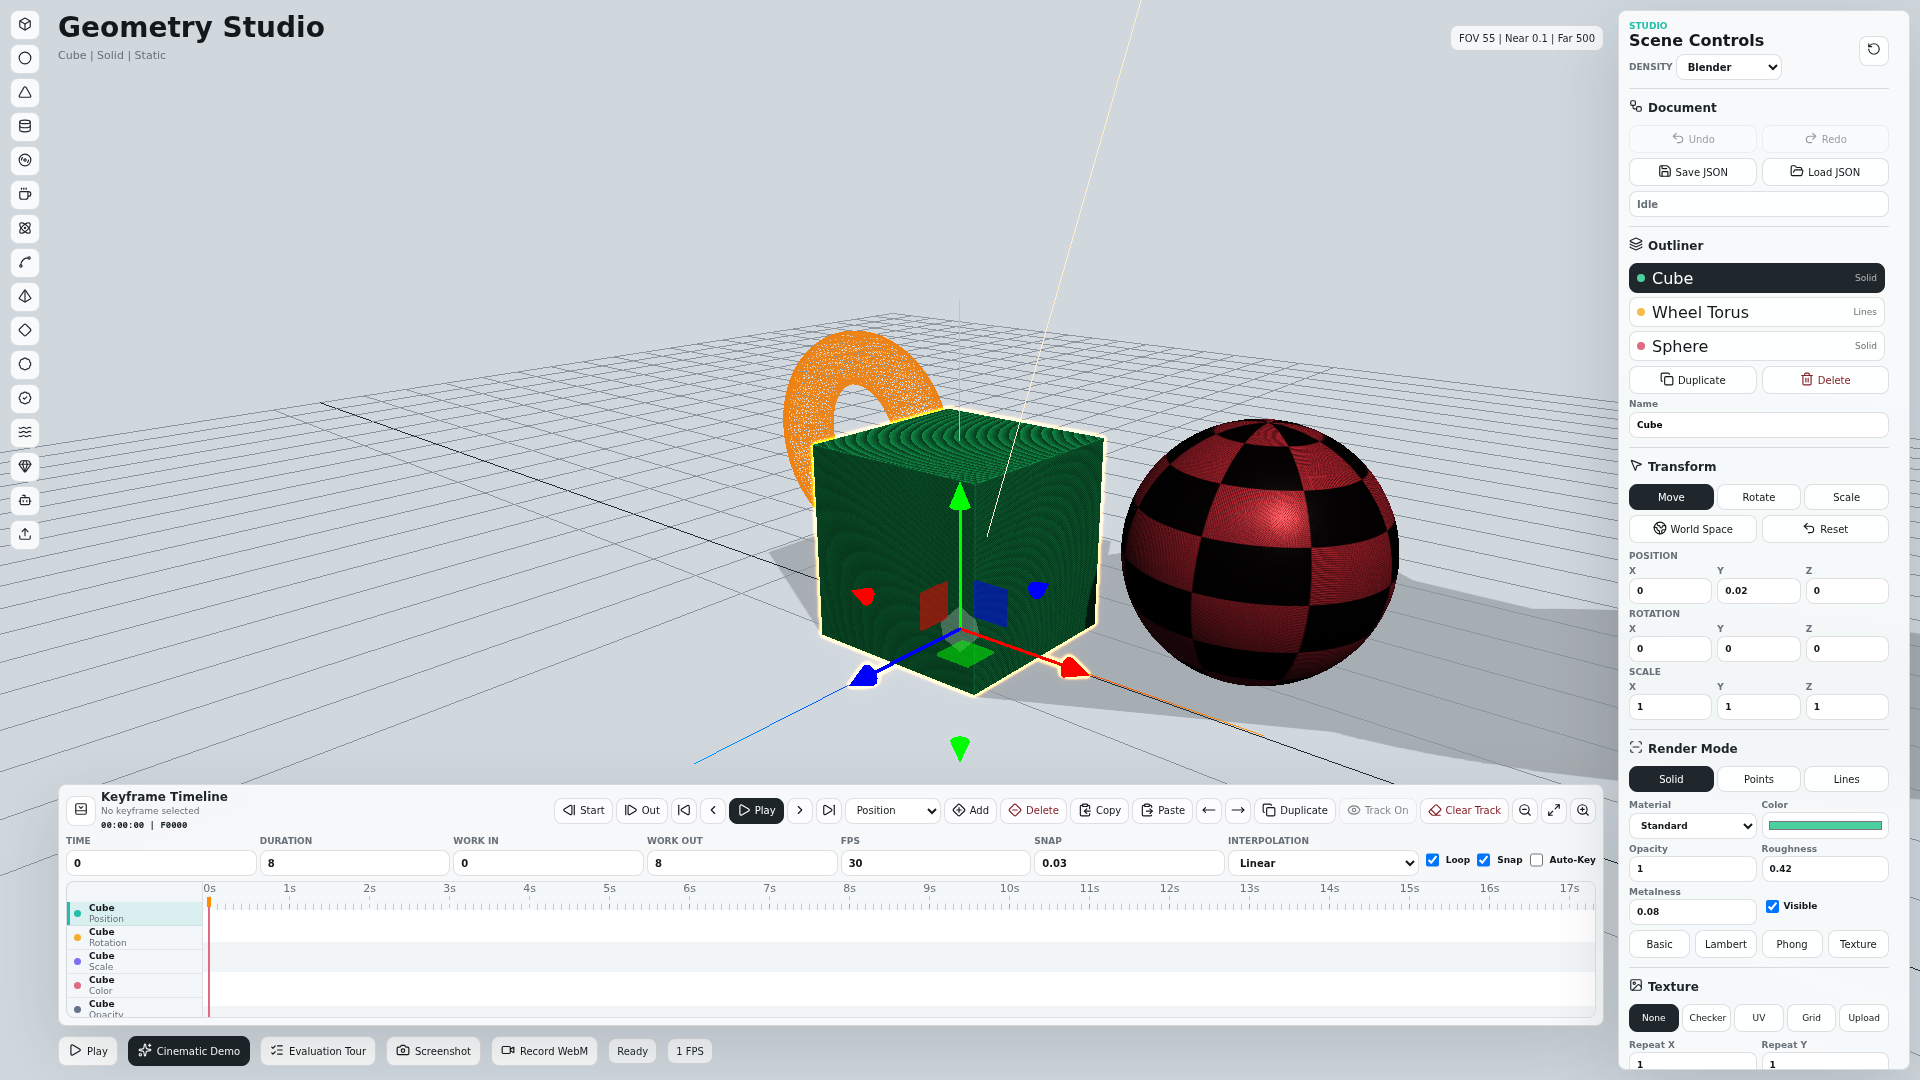
\includegraphics[width=\linewidth]{screenshots/01-default-studio.png}
\caption{Default Geometry Studio scene with primitive geometry, render modes,
inspector controls, transform gizmo, grid, and timeline dock.}
\end{figure}

\begin{figure}[htbp]
\centering
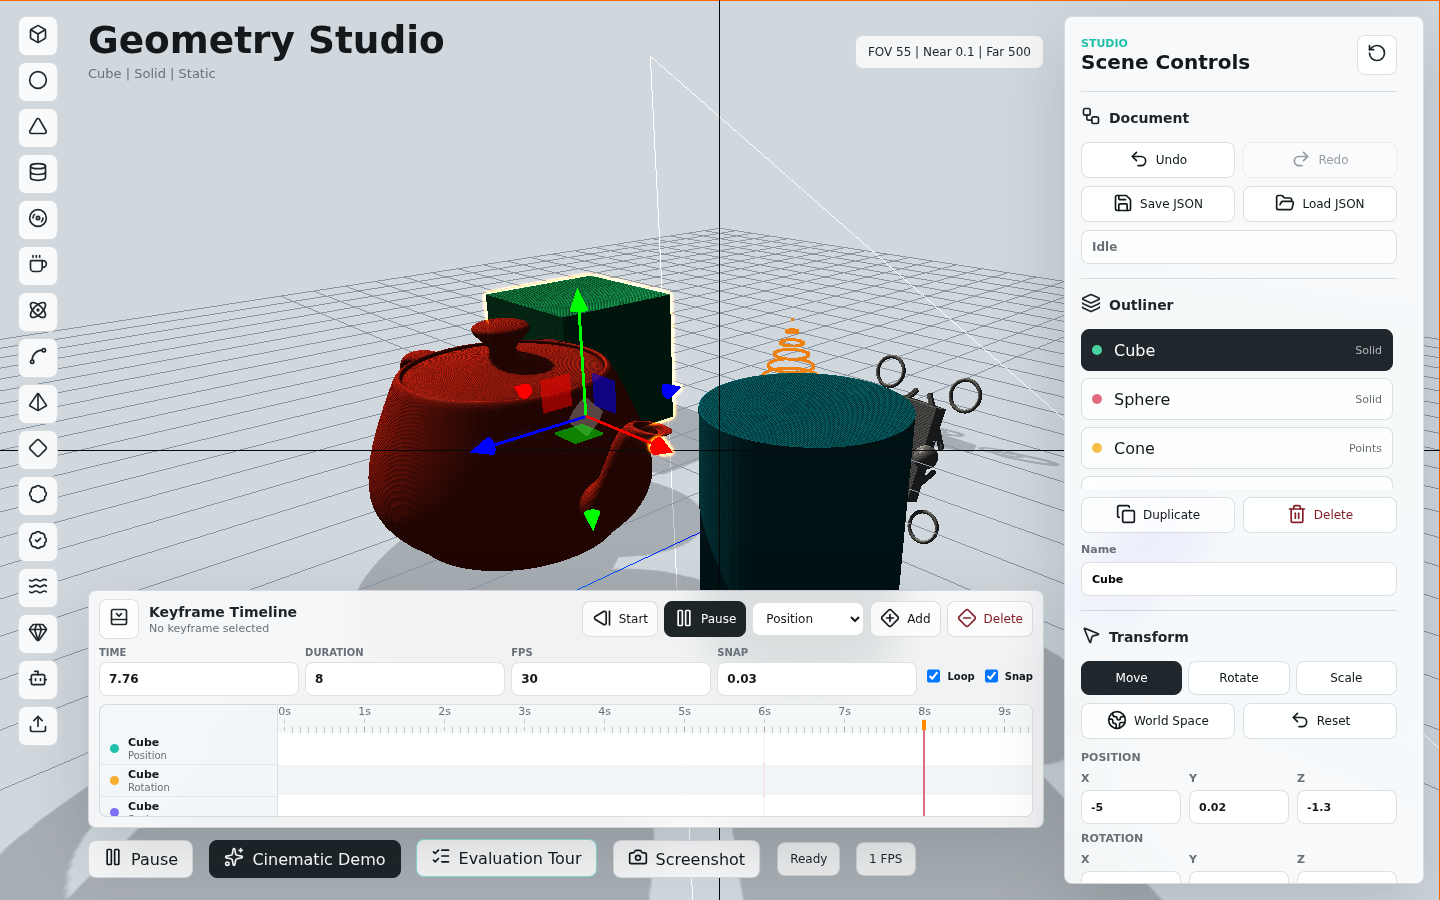
\includegraphics[width=\linewidth]{screenshots/02-evaluation-tour.png}
\caption{Evaluation Tour scene showing required primitives, shadows, camera
frustum helper, lighting helpers, and multiple rendering modes.}
\end{figure}

\begin{figure}[htbp]
\centering
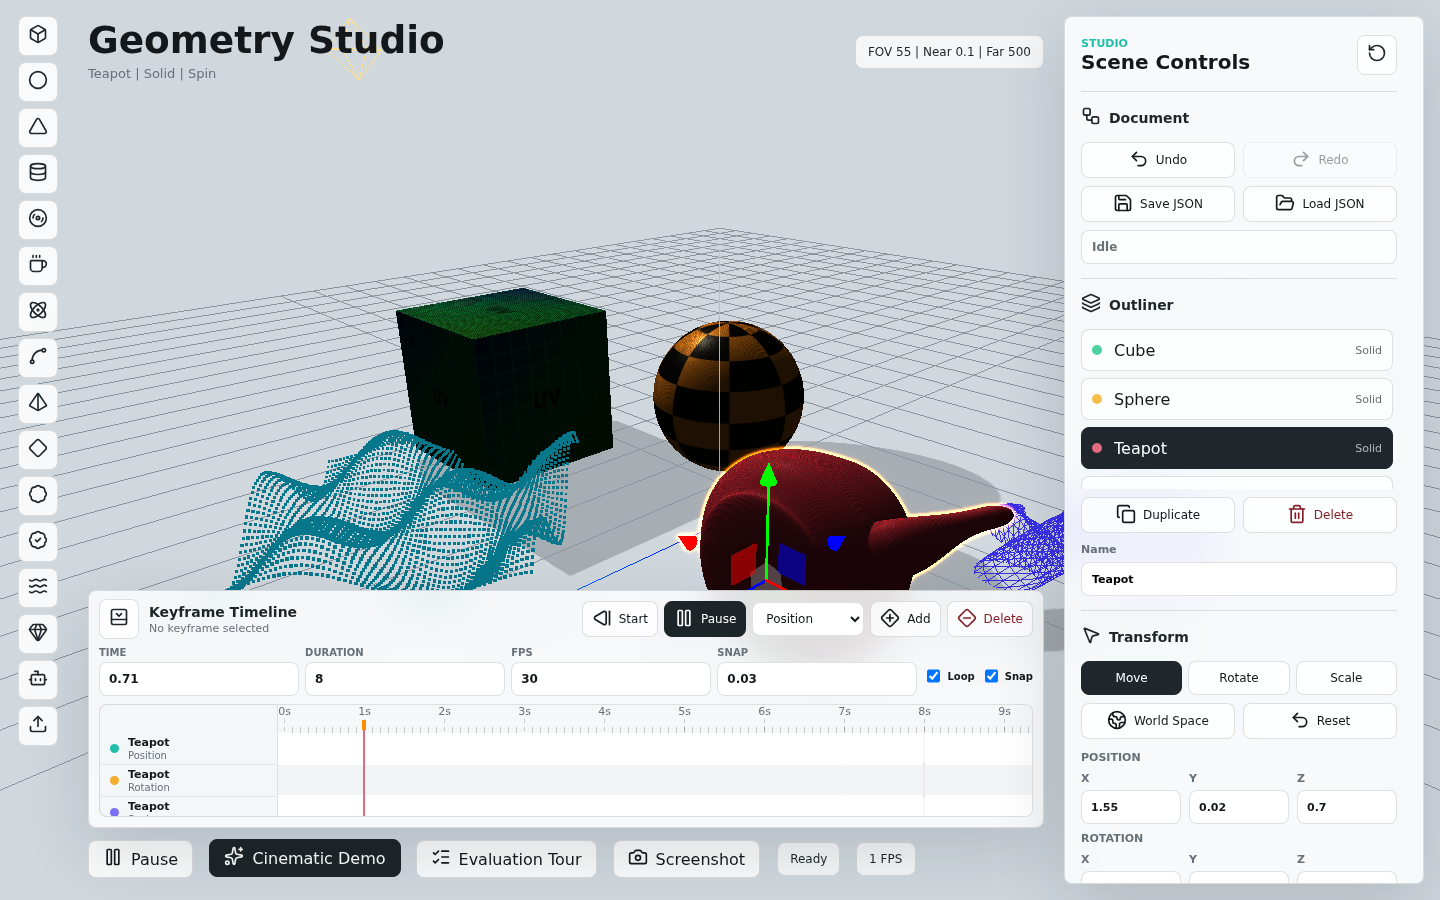
\includegraphics[width=\linewidth]{screenshots/03-cinematic-rendering.png}
\caption{Cinematic rendering demo with mixed primitives, textures, point/line
rendering, lighting, shadows, and animation playback.}
\end{figure}

\begin{figure}[htbp]
\centering
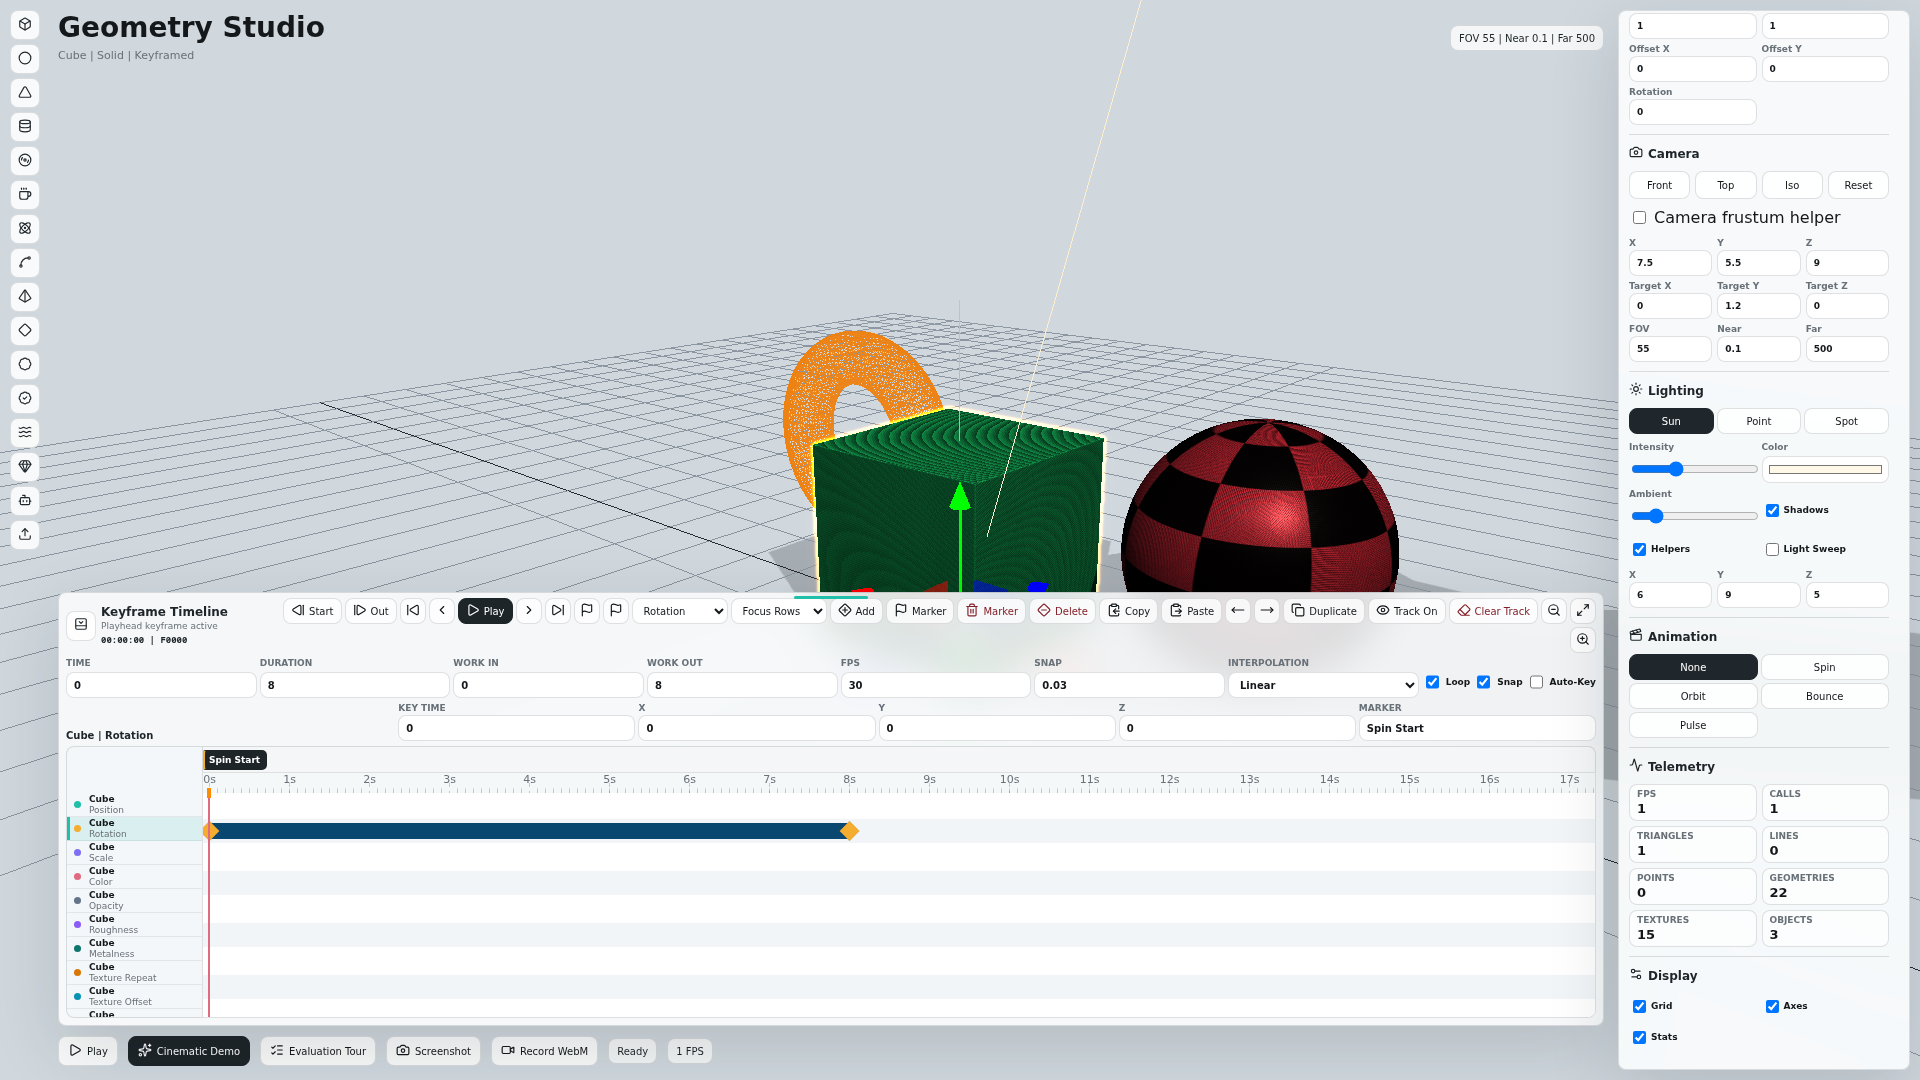
\includegraphics[width=\linewidth]{screenshots/04-keyframe-timeline.png}
\caption{Resizable keyframe timeline showing editable track rows, markers, and
selected keyframe values in the timeline workflow.}
\end{figure}

\begin{figure}[htbp]
\centering
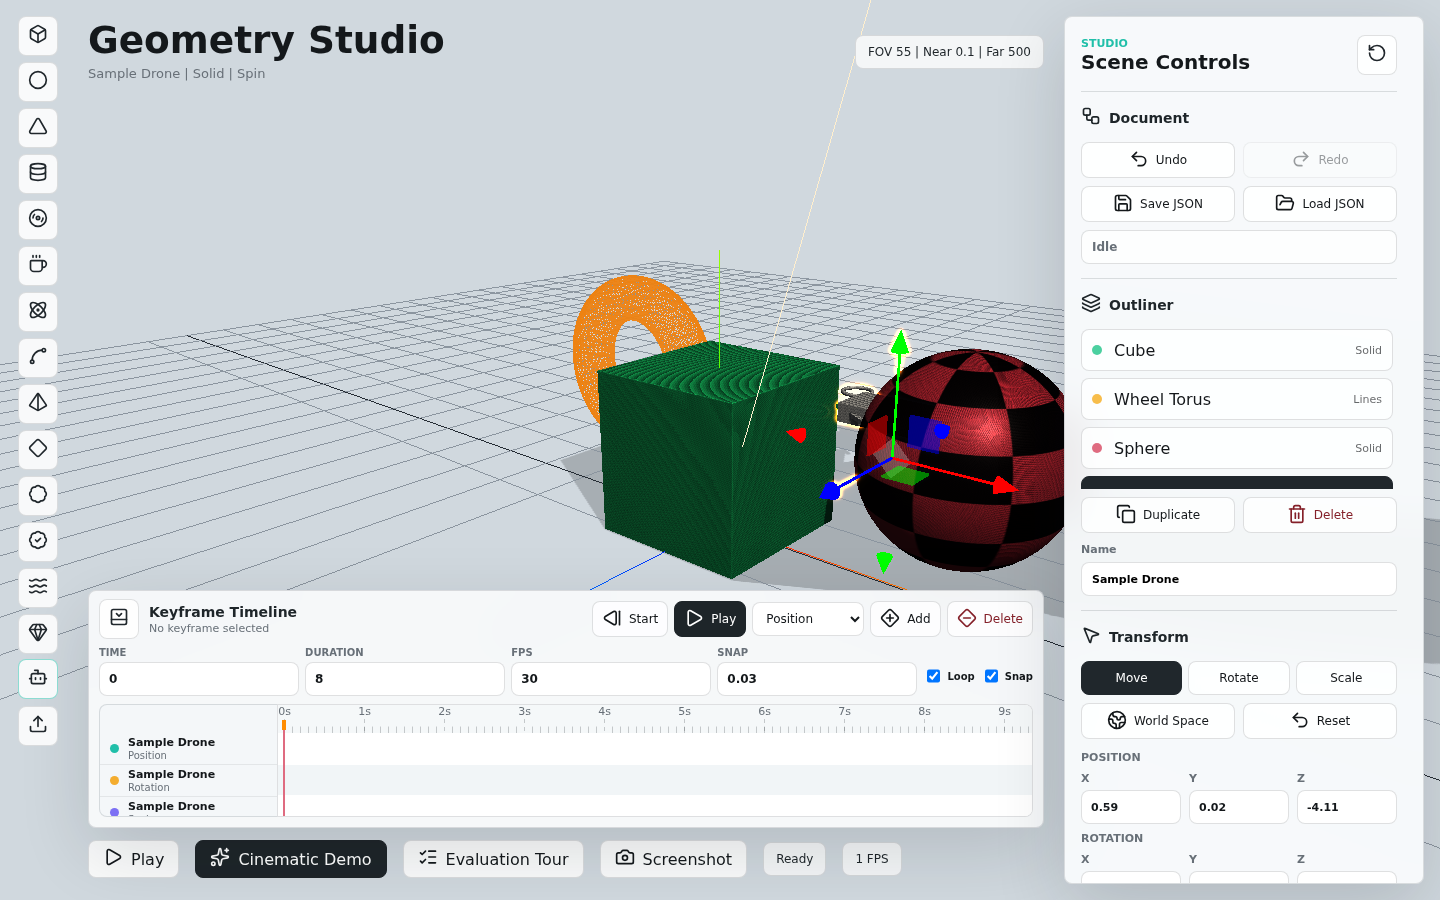
\includegraphics[width=\linewidth]{screenshots/05-sample-model-workflow.png}
\caption{Built-in sample model workflow demonstrating model-style objects in
the same outliner, transform, render, and animation system.}
\end{figure}

\begin{figure}[htbp]
\centering
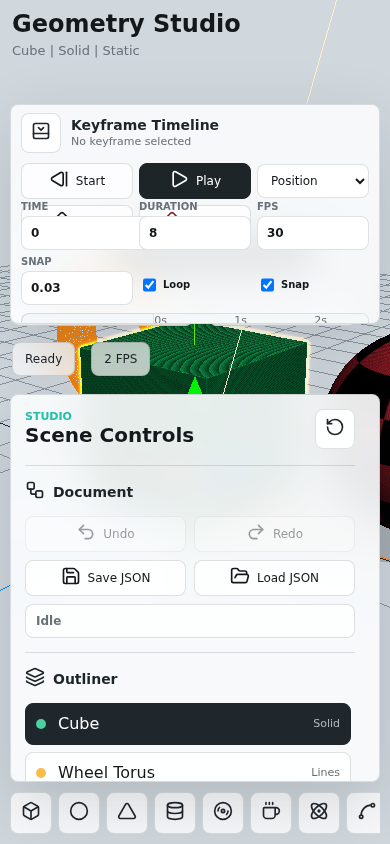
\includegraphics[width=0.55\linewidth]{screenshots/06-mobile-responsive-layout.png}
\caption{Responsive mobile layout with timeline, inspector, viewport, and
horizontal tool rail.}
\end{figure}

\begin{figure}[htbp]
\centering
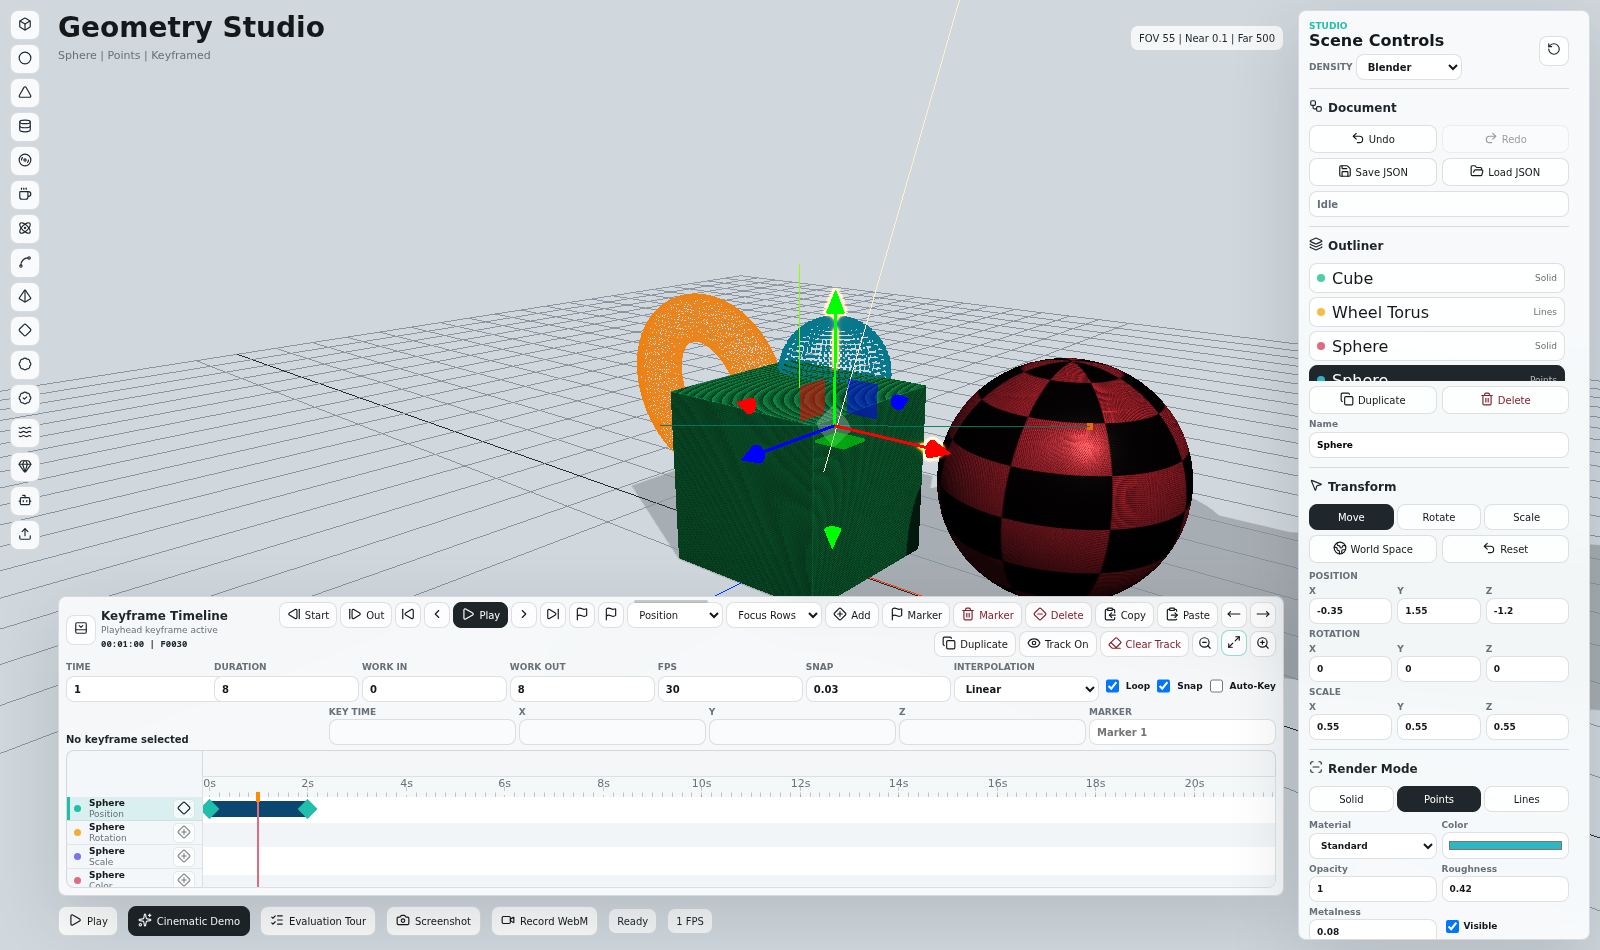
\includegraphics[width=\linewidth]{screenshots/07-motion-path-timeline.png}
\caption{Position keyframes with the selected object's viewport motion path,
showing the spatial interpolation from one keyed position to the next.}
\end{figure}

\begin{figure}[htbp]
\centering
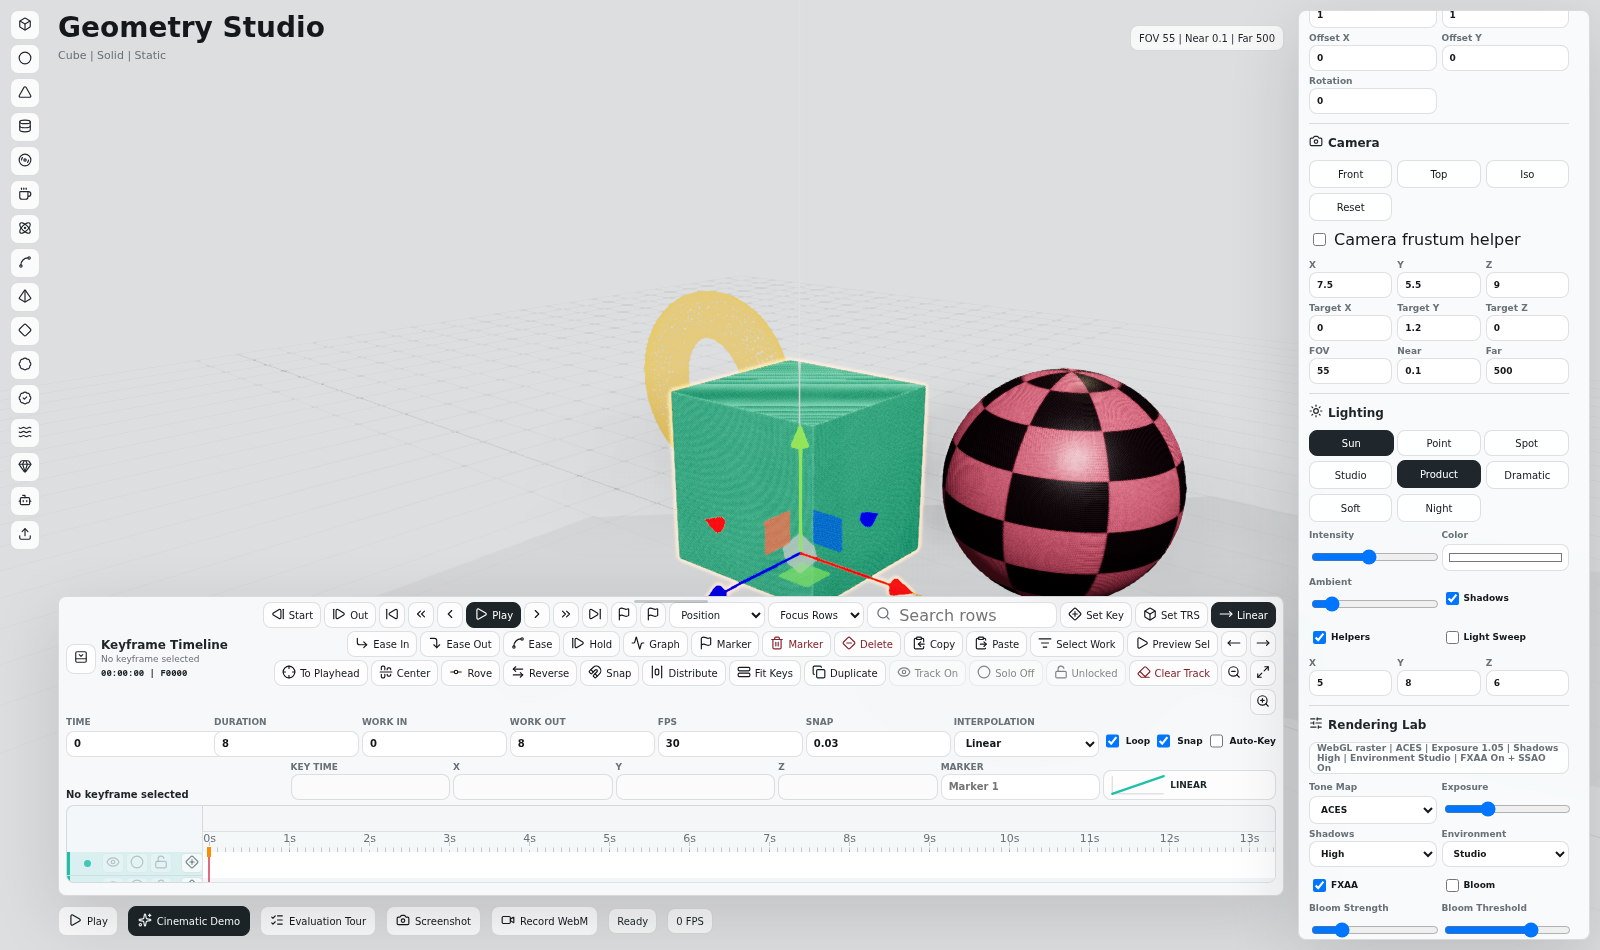
\includegraphics[width=\linewidth]{screenshots/08-rendering-lab-lighting.png}
\caption{Rendering Lab with Product lighting, FXAA, SSAO, tone mapping,
environment lighting, and the direct-light preset controls visible in the
inspector.}
\end{figure}

\section{Source Architecture}

The upgraded source code is split into focused modules:

\begin{table}[h]
\centering
\begin{tabular}{>{\ttfamily}p{0.34\linewidth}p{0.56\linewidth}}
\toprule
Module & Responsibility \\
\midrule
editor/types.ts & Shared application types such as SceneEntry, LightRig, and SceneDocument. \\
editor/documents.ts & Scene JSON serialization and validation. \\
editor/commands.ts & Undo/redo snapshot history. \\
animation/timelineSchema.ts & Timeline defaults, validation, migration, snapping, and object-track helpers. \\
animation/timelineEditing.ts & Pure keyframe editing operations such as source resolution, copy, paste, duplicate, frame nudge, and numeric keyframe edits. \\
animation/interpolation.ts & Shared per-keyframe evaluator for Hold, Linear, and Easy Ease timing. \\
animation/timelinePlayer.ts & Applies object Position, Rotation, and Scale tracks directly to scene objects. \\
scene/primitives.ts & Primitive geometry, extra shapes, labels, and built-in sample model. \\
scene/materialPresets.ts & PBR and legacy material preset definitions. \\
scene/materials.ts & Materials, texture presets, and solid/point/line visual construction. \\
scene/lights.ts & Stage, light rig, shadows, helpers, and light sweep. \\
scene/lightingPresets.ts & Named direct-light rigs for Studio, Product, Dramatic, Soft, and Night lighting. \\
scene/importers.ts & GLB, GLTF, OBJ, and STL import pipeline. \\
renderer/environment.ts & Generated PMREM environment lighting controller. \\
renderer/pipeline.ts & WebGLRenderer, EffectComposer, FXAA, SSAO, Bloom, Vignette, OutlinePass, and resize handling. \\
renderer/postProcessing.ts & Post-processing defaults, normalization, application, and status labels. \\
animation/timeline.ts & Legacy procedural animation helper retained for compatibility. \\
ui/template.ts & DOM template for the editor UI. \\
ui/density.ts & UI density loading, persistence, and root layout mode application. \\
ui/timelinePanel.ts & Adapter between the timeline UI component and editor commands. \\
utils/resourceTracker.ts & Explicit disposal of geometries, materials, textures, and URLs. \\
\bottomrule
\end{tabular}
\caption{High-level source structure.}
\end{table}

\section{Rendering and Performance Considerations}

The renderer is configured for WebGL2 with ACES tone mapping, sRGB output color
space, configurable soft shadows, generated PMREM environment lighting, and an
EffectComposer chain for SSAO, Bloom, Vignette, selected-object outlines, FXAA,
and final output conversion. Resize handling uses the canvas client size and
caps the drawing buffer pixel count to avoid excessive GPU load on high-DPI
displays. SSAO and Bloom use smaller internal buffer budgets to preserve
interactive performance.

The project explicitly disposes geometries, materials, textures, and object URLs
when objects are rebuilt or removed. This follows standard Three.js resource
management practices and reduces the risk of memory leaks during long editing
sessions.

\section{Future Improvements}

The current release focuses on a stable real-time WebGL editor. The following
items are reasonable future extensions after the submitted release.

\begin{enumerate}
  \item \textbf{Path-Traced Preview}: evaluate a separate progressive still
  preview using a GPU path-tracing library. This should remain optional because
  the main editor is designed for real-time rasterized interaction.
  \item \textbf{Advanced Curve Editing}: add Bezier handle editing in the value
  graph while preserving the current simple keyframe workflow.
  \item \textbf{Nested Model Tracks}: allow imported model children to expose
  their own transform and material tracks.
  \item \textbf{Video Export Options}: add richer WebM settings and optional GIF
  export if browser support is reliable.
\end{enumerate}

\section{Testing}

The project includes automated browser tests with Playwright:
\begin{itemize}
  \item Startup rendering and non-empty canvas verification
  \item Toolbar and inspector visibility
  \item Object creation
  \item Render mode switching
  \item Responsive mobile layout smoke test
  \item Undo and redo
  \item Scene JSON loading
  \item Keyframe timeline creation and JSON save verification
  \item Auto-Key initial value seeding
  \item Rendering Lab FXAA, SSAO, Bloom, and Vignette controls
  \item Direct lighting preset persistence
  \item Evaluation Tour activation
\end{itemize}

The main verification commands are:
\begin{verbatim}
npm run typecheck
npm run build
npm run test:smoke
\end{verbatim}

\section{How to Run}

To run from source:
\begin{verbatim}
cd Geometry_Studio/Source
npm install
npm run dev
\end{verbatim}

To run the static release:
\begin{verbatim}
cd Geometry_Studio/Release
python3 -m http.server 8080
\end{verbatim}

Then open:
\begin{verbatim}
http://localhost:8080
\end{verbatim}

\section{Conclusion}

Geometry Studio satisfies the project requirements for 3D geometry,
rendering modes, perspective projection, affine transformations, lighting,
shadows, texture mapping, model loading, and animation. The upgraded version
also adds scene persistence, undo/redo, import progress, drag-and-drop, telemetry,
Rendering Lab controls, direct-lighting presets, post-processing effects, an
Evaluation Tour, screenshot and WebM export, and a modular source architecture.
These features make the project easier to evaluate, easier to maintain, and more
impressive as a complete computer graphics demonstration.

\end{document}
